%!TEX root = Constructive Alignment for Introductory Programming.tex

\chapter{Discussion} % (fold)
\label{cha:discussion}

\graphicspath{{Figures/Discussion/}}

\cref{cha:guiding_principles} presented twelve principles that extend the core principle of constructive alignment to help create a student-centred learning environment centred around constructive learning theories. These principles were then used to guide the creation of the model of constructive alignment for introductory programming presented in \cref{cha:approach}. Chapters \ref{cha:example_impl} and \ref{cha:supporting} provided details of two example units implemented using this approach, and the supporting resources used to assist students in constructing appropriate knowledge. With \cref{cha:evaluation} providing an analysis of the evolution of the approach and assessment criteria, through iterative action research, and evaluations of issues students faced and the use of the Doubtfire tool for tracking student progress. 

This chapter discusses the overall experience of developing and delivering units using this approach. \sref{sec:general_applicability_of_constructive_alignment} provides support for Biggs' claim that for the general applicability of constructive alignment, providing some illustrations of how other units could be implemented using the approach from \cref{cha:approach}. \sref{sec:approach_in_relation_to_previous_work} relates the approach presented back to the original proposal of constructive alignment with portfolio assessment. \sref{sec:principles_in_review} and \sref{sec:approach_in_review} discuss the importance of each of the guiding principles from \cref{cha:guiding_principles} and the aspects of the approach from \cref{cha:approach}. Challenges for the wider adoption of this approach are then discussed in \sref{sec:challenges_for_wider_adoption}, before a final discussion of the approach overall. The chapter then concludes with some closing comments in \sref{sec:disc_summary}.

\clearpage

\section{General Applicability of Constructive Alignment} % (fold)
\label{sec:general_applicability_of_constructive_alignment}

Biggs' original proposal of constructive alignment concluded with the following question:

\begin{quote}
	``Can the principle of constructive alignment be generalised from the context of in-service teacher education?'' \citet{Biggs:1996c}
\end{quote}

While others have applied the core principle of constructive alignment, as discussed in \cref{cha:background}, this work has identified additional principles to help recreate the ``web of consistency'' that provided the inspiration for \citet{Biggs:1996c,Biggs:1999} constructive alignment. The twelve principles stated in \cref{cha:guiding_principles} underpin the approach to constructive alignment described in \cref{cha:approach} which, together with the principles, guided the design, development, and delivery of the units described in \cref{cha:example_impl}. The results? A supportive, student-centred, teaching and learning environment in which, to use the words of \citet{Biggs:2007} (p.51), students consistently ``\emph{stun}'' teaching staff with the ``\emph{rich and exciting}'' work they demonstrate in their portfolios.

As outlined in \cite{Biggs:1996c}, the model of constructive alignment makes intuitive sense, and comes together as a whole when the following conditions are met.
\begin{enumerate}[noitemsep,nolistsep]
	\item Teaching staff are clear about the \emph{intended learning outcomes}.
	\item Assessment criteria are provided to indicate how these outcomes can be met at various levels of achievement, forming a hierarchy from barely satisfactory to most acceptable.
	\item Students are required to perform activities that are likely to elicit the required understandings.
	\item Students provide evidence that their learning has matched the stated outcomes.
\end{enumerate}

\cref{cha:approach} demonstrated how the guiding principles described in \cref{cha:guiding_principles} can be applied to create an approach to teaching introductory programming that meet, and in many regards go beyond, these conditions. The processes described started with the clear expression of intended learning outcomes, with the development of assessment criteria providing the required performance objectives required for different grade outcomes. The development of teaching and learning activities aimed to provide students with tasks likely to engage them in activities that will enable them to construct appropriate understandings, and produce evidence they can include to demonstrate their newly gained knowledge. This evidence could then be collected together and presented in student portfolios as a means of demonstrating how the stated objects had been met.

Therefore, the approach presented in \cref{cha:approach}, along with the example implementation discussed in Chapters \ref{cha:example_impl} to \ref{cha:evaluation}, provide additional support for Biggs' claim that constructive alignment using portfolio assessment can be generalised to a range of educational contexts. 

The general applicability of constructive alignment gives rise to the question: Can the approach presented in \cref{cha:approach} be used beyond the context of introductory programming? We believe so. In fact this approach has been used to implement a range of units, as outlined in the following list, each with similar positive results.

\begin{itemize}[noitemsep,nolistsep]
	\item Artificial Intelligence for Game used intended learning outcomes related to the use of Artificial Intelligence in creating immersive gaming experiences. Student portfolios included a number of programs to demonstrate various techniques, with higher grades demonstrating the application of learnt concepts in the development of a program of the students own invention.
	\item Concurrent Programming covered the use and implementation of concurrency control mechanisms such as semaphores, barriers, and channels. Portfolios included implementations of these utilities, along with programs demonstrating solutions to classic synchronisation problems.   
	\item Enterprise Software Development involved the use of a range of software tools to implement larger, multi-tier, solutions to business scenarios. Portfolios included demonstrations of various technologies, architectural designs, and technical demonstrations of core components of these designs.
	\item Games Programming introduced concepts related to game design, and the implementation of game engine concepts. Portfolios included demonstrations of various programming techniques and optimisations related to game development, with students implementing game prototypes for higher grades.
	\item Mobile Software Development explored the implementation of software for mobile devices, and associated usability issues. Students applied concepts they learnt in the creation of their own programs for higher grades.
	\item Research Project involved undergraduate students undertaking and documenting a small research project. Portfolios included artefacts created from the research project, which consisted of, at least, a research proposal and plan, research report, artefacts associated with an oral presentation, and a learning summary report. 
\end{itemize}

In each case the units involved incorporated the principles from \cref{cha:guiding_principles}, with the central role of programming paradigms (\Pref{itm:paradigm}) in the development of introductory programming units being adjusted to focus on key aspects relevant for each unit. The use of portfolio assessment in each case meant that similar, in many cases identical, assessment criteria were able to be used.

While all of these units are technical in nature, we believe the approach can also be applied to non-technical units. The large majority of processes described in \cref{cha:approach}, and their associated guidelines, are applicable for both technical and non-technical units. Assessment criteria is where this is likely to differ. Programming units involve a significant focus on functioning knowledge, involving the practical application of concepts learnt to problem solving and the creation of computer software. The resulting assessment criteria then promote the use of this functioning knowledge in a creative context, and the submission of the resulting artefacts to be eligible for high grades. Where a unit primarily focuses on declarative knowledge such assessment criteria will not be applicable. In these contexts alternative assessment criteria would be required, with the aim of students demonstrating relational levels of understanding in some creative context enabling students to explore aspects of the unit they find most interesting. For example, a unit may require students to undertake wider reading and present their findings to the class or in an extended literature review.

The use of the approach from \cref{cha:approach} would also be particularly well suited to assess learning outcomes for units that include significant use of group work, such as with team-based final year capstone projects. In these unit students work as part of a team, with obvious challenges in assessing the learning outcomes from individual students as final work products are a team effort. Using the approach from \cref{cha:approach} it would be possible to create a learning environment for these units in which:
\begin{itemize}[noitemsep,nolistsep]
	\item Intended learning outcomes capture the required technical and teamwork skills and understandings students needed to demonstrate to successfully complete the unit.
	\item Assessment criteria indicate how these outcomes needs to be demonstrated in order to achieve different grade outcomes.
	\item Students engage in teamwork activities, which are likely to elicit the required outcomes.
	\item Each students collects evidence that they have met all of the intended learning outcomes, aligns their evidence in a Learning Summary Report, and presents this for assessment.
\end{itemize}

In this way, each student's grade would reflect how well they, as individuals, had met the intended learning outcomes. Creating such a scheme would require the embodiment of all principles stated in \cref{cha:guiding_principles}, particularly the need to trust and empower students in their learning (\Pref{itm:theory_y}).

One place where we differ from the recommendations of \citet{Biggs:2007} is in the use of portfolios for larger class sizes. Incorporating frequent formative feedback, tracked by the online Doubtfire tool, made it possible to use portfolio assessment with classes in excess of 300 students (323 students completed the introductory programming units in iteration 8). The frequent formative feedback meant that student work submitted in their portfolios had \emph{already} been checked, possibly multiple times, and if completed successfully this had been indicated in the Doubtfire tool. As a result, the majority of student work did not need to be re-checked in their final portfolios, and grades could be quickly determined. 

Reflections from teaching staff indicate that the resulting process enabled student portfolios to be assessed in significantly less time than it took to assess the previously used exams -- which consisted of multiple choice, short answer, and coding questions. Given this, and ongoing improvements through reflective practice, it is also believed that the use of portfolio assessment could scale to significantly larger class sizes.

% subsection general_applicability_of_constructive_alignement (end)


\clearpage
\section{Approach in Relation to Previous Work on Constructive Alignment} % (fold)
\label{sec:approach_in_relation_to_previous_work}

Previous work on applying constructive alignment, as reported in the structured literature review from \cref{cha:background}, has predominantly seen the application of constructive alignment as simply the task of staff aligning teaching and learning activities with the unit's intended learning outcomes. This differs vastly from the view of constructive alignment presented in this thesis, where constructive alignment is seen as a much greater shift in educators understanding and approach to teaching and learning, one that is centred upon the principles outlined in \cref{cha:guiding_principles}. When constructive alignment is seen in this way, the resulting teaching and learning environment \emph{must} shift from a teaching-centred to a student-centred focus, with all aspects working together to guide and support students in the construction of their own knowledge.

This change in conception requires an adjustment to fundamentally held notions of effective education and its assessment. The continued use of arbitrarily weighted assignments and exams is ineffective in communicating the focus on learning and understanding. Restrictive assessment practices, the result of largely Theory-X dominated views of motivation, limit student opportunities, confining them to pre-set bounds defined as effective learning by teaching staff. By trusting and empowering students through the use of open assessment practices, guided by a Theory-Y view of motivation, these artificial constraints disappear and students are free to use their imagination and creativity. The results, as originally reported by \citet{Biggs:2007} and supported by our experiences outlined in \cref{cha:evaluation}, are portfolios that are truly amazing. 

Prior to adopting the approach outlined in \cref{cha:approach}, the staff involved in teaching the units discussed in \cref{cha:example_impl} often felt that assessment was a negative experience. Marking assignments and exams identified, often for the first time, a large range of student misconceptions. The illusion that lectures had been effective in transferring knowledge to students disappeared, but too late to effect learning outcomes. This was further reinforced with potential arbitrary weights of assignments and exams often resulting in cases where teaching staff felt the student results did not match the knowledge, or lack thereof, that they had demonstrated in the final assessment tasks. It is not surprising that this form of assessment often resulted in disappointment.

All of this changed with the shift in approach. Final student assessment becoming a positive and rewarding experience for teaching staff. Use of frequent formative feedback meant that students misconceptions were addressed often, allowing teaching staff to direct students and guide them to better understand unit concepts. ``Assessments'' were no longer final, so students were encouraged and rewarded for incorporating feedback they received, with each student receiving individual feedback based upon their current level of understanding. Assessment criteria provided a means for teaching staff to set expectations, while still providing opportunities for students to pursue their own interests and to use their imagination and creativity. So final assessment did not hold any \emph{negative} surprises. Portfolios provided an opportunity for students to ``\emph{show off}'' what they had learnt. Where students had achieved Distinction and High Distinction results, these portfolios often went well beyond staff expectations, making assessment a rewarding experience for teaching staff as students demonstrated just how much they had been able to achieve.

It is hard not to draw parallels between these different approaches to education and different software development life-cycle models. Traditional assessment approaches, based upon assignments and exam, can be likened to the Waterfall approach. Teaching and learning activities are delivered in sequence, with little feedback from students. When feedback is provided on summative assignments it is often overlooked \cite{Black:1998}, as students focus on the grade they achieved rather than on opportunities for deeper learning. The accumulated misunderstandings are then ever apparent in the final examination. In contrast, the iterative process outlined in \cref{cha:approach} is more akin to processes in Agile software development. Students and staff interact frequently, enabling staff to guide students with the focus being clearly on their learning during the teaching period. Final summative assessment in student portfolios demonstrate to what level students have been able to achieve stated unit outcomes, with higher grades indicating a demonstration of deeper understanding.

% section approach_in_relation_to_previous_work (end)

\section{Principles in Review} % (fold)
\label{sec:principles_in_review}

\cref{cha:guiding_principles} provided twelve principles used to guide the creation of the student centred approach to teaching introductory programming presented in \cref{cha:approach}. While each principle has its own individual merits, we believe that they are all required to work together in order to achieve the outcomes presented. This section draws upon the experiences of teaching staff, as reported in \cref{cha:evaluation}, to discuss the potential impact of failing to address each of these principles on the overall learning environment. The following list outlines how the principles are designed to work together, as a reference for this discussion.

\begin{itemize}[noitemsep,nolistsep]
	\item Constructive learning theories are central, with everything in the system aiming to help students construct appropriate knowledge, to enable them to think and act as experts. (\Pref{itm:construct})
	\item Activities and resources aim to align with stated intended learning outcomes, which students must demonstrate they have achieved. (\Pref{itm:align})
	\item Formative feedback supports learning throughout the teaching period, with summative assessment qualitatively evaluating how well students have achieved learning outcomes at the end of the unit. (\Pref{itm:formative})
	\item Delivery focuses on communicating important aspects, while providing resources to support students as they need additional details. (\Pref{itm:focus})
	\item Communicating high expectations helps to encourage students to excel, and instil in them a sense of achievement when they succeed. (\Pref{itm:expectations})
	\item Actively supporting students efforts helps each student to achieve the their full potential.  (\Pref{itm:support})
	\item Empowering students by allowing them to manage their own learning helps students become life-long learners. (\Pref{itm:theory_y})
	\item Being agile and willing embraces opportunities for improvement. (\Pref{itm:agile})
	\item Reflective practice helps recognise opportunities for improvement, for both teaching staff and students. (\Pref{itm:reflect})
	\item Having a central focus, such as a programming paradigm, helps provide coherence to the intended learning outcomes and guide the delivery strategy for the unit.  (\Pref{itm:paradigm})
	\item Communicating concepts to students helps them build the knowledge they need to act as experts. (\Pref{itm:concepts})
	\item Always using tools as intended, such as authentic use of programming languages, helps to ensure student experiences develop appropriate knowledge. (\Pref{itm:authentic})
\end{itemize}

\subsection{Constructive Learning Theories} % (fold)
\label{sub:constructive_learning_theories}

\pref{itm:construct} plays a central role in providing the motivation for all of the other principles. Following the mechanisms underlying this approach without adjusting the underlying view of education is likely to be challenging. Where understanding is not seen as being constructed by individual learners there is little need to attempt to create teaching and learning activities that actively engage students. Effective teaching becomes a matter of effectively delivering the required knowledge, resulting in teacher-centred activities coming to the fore. 

Adopting constructive learning theories in teaching and learning activities addresses only part of the overall teaching and learning environment. The central role of assessment implies that these theories need to extend beyond teaching and learning activities to assessment. Applying traditional assignment and exam assessment schemes limits the opportunity for students to demonstrate their understanding in a way that is meaningful to them. Given their role in constructing their knowledge, they are best situated to determine what represents the best demonstration of their understanding. Implementing the other principles without adopting more flexible assessment approaches is likely, therefore, to limit the effectiveness of the learning environment overall as students are limited by the assessment approach.

While the core ideas of constructivism need to be incorporated, \cref{cha:guiding_principles} argued that constructive learning theories needed to be moderated with pragmatic aspects to avoid unproductive discovery learning. While knowledge transmission cannot be achieved, approached based on discovery learning have been shown to be ineffective, as was found in the early iterations discussed in \cref{cha:evaluation}. 

These competing views can be best thought of as a continuum based upon communication; from knowledge transmission with objectivist learning theories, to discover learning with constructivist theories. This continuum is shown visually in \fref{fig:balanced_constructivism}, which depicts the underlying concepts that drive the actions of teaching staff when they hold these views. At the objectivist end of the continuum communication is key, and teaching staff work to communicate all of the aspects students need to understand. This view is teacher-centred as the teacher communicates the required understanding for students to passively absorb. At the other end, the extreme constructivist view discards any value in communication, instead students are placed in situations and asked to ``discover'' the knowledge themselves. Adopting either of these extreme positions is not likely to result in an effective, student-centred, learning environment.

\begin{figure}[htbp]
	\centering
	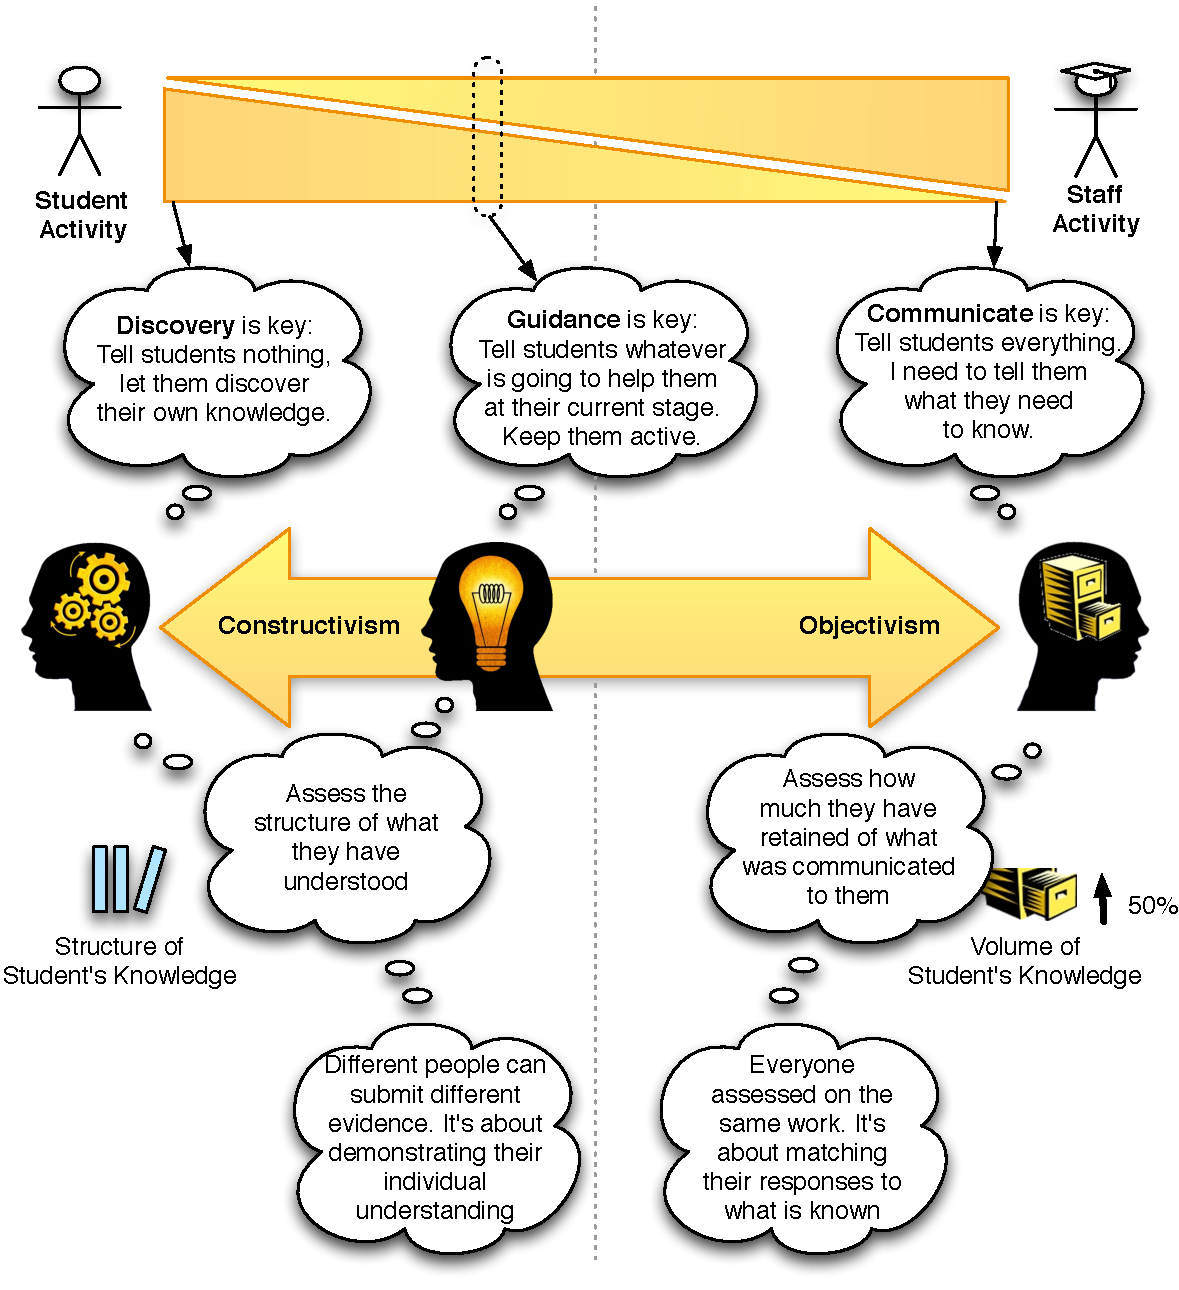
\includegraphics[width=\textwidth]{BalanceConstructivism}
	\caption{Thoughts that guide teaching staff at either end of the constructivism-objectivism continuum. \cref{cha:guiding_principles} advocates a pragmatic approach to constructivism, somewhere on the constructivist side of the continuum. }
	\label{fig:balanced_constructivism}
\end{figure}

\pref{itm:construct} requires a middle ground approach. To embrace this approach, educators need to accepts the central role of the student in constructing their own knowledge, while also accepting that communication can be a powerful tool to help guide this construction. Communication then becomes a valuable tool, with teaching staff being encouraged to communicate as little or as much as is \emph{needed} by the students at that stage of their learning. Communication is not used to transfer knowledge, but to help guide students so that they may see how viable knowledge can be shaped.

Reflections from the evaluation of the unit deliveries across the various iterations in \cref{cha:evaluation} provide some support for taking this middle ground approach. Teaching staff attribute many of the failings of the object oriented programming unit in Iteration 2 to an overly zealous application of constructive learning theories, and discovery learning. Moving back from these extreme, to a more moderate application of constructive learning theories addressed this situation in later iterations, and as staff expertise in guiding students improved, so did student results.

% subsection constructive_learning_theories (end)

\subsection{Aligned Curriculum} % (fold)
\label{sub:disc_aligned_curriculum}

Aligning all aspects of the teaching and learning environment (\Pref{itm:align}) makes good intuitive sense. Failing to address this principle is likely to result in one of three potential outcomes based upon the alignment between the three component parts: teaching and learning activities, assessment tasks, and intended learning outcomes.

\begin{enumerate}[noitemsep,nolistsep]
	\item Where assessment aligns to intended learning outcomes, but activities do not, students are likely to be unprepared for the assessment tasks. While assessment does define the curriculum for the students, activities provide a means of preparing them for this assessment. 
	\item Where activities align to intended learning outcomes, but assessment does not, students may build appropriate knowledge but the assessment is unlikely to identify this, with final student results failing to represent their ability to meet the intended learning outcomes. 
	\item Where neither assessment nor activities align with intended learning outcomes, students are not likely to learn what was intended in terms of their overall degree programme outcomes. While students may effectively learning something valuable, and the assessment appropriately report this, the misalignment is likely to cause issues for students in later units, or professional life, where they are required to rely upon the intended learning outcomes of the unit.
\end{enumerate}

Alignment is, therefore, a critical aspect in creating an effective learning environment. By aiming to achieve consistency between teaching and learning activities, assessment tasks, and intended learning outcomes, teaching staff provide students with the greatest opportunity to learn the required knowledge, in an effective manner. 

It is also critical to understand that students must also be involved in this alignment process. The interplay between \pref{itm:construct} and \pref{itm:align} means that students, not staff, are in the best position to report on how teaching and learning activities and assessment tasks aligned with the intended learning outcomes. Students followed the planned activities, carried out the assessment tasks all of which helped them in the construction of their knowledge. It is the students, therefore, who truly know how these activities aligned.

The implication of this is that there is not likely to be one measure of alignment for a set of teaching and learning activities. Each students learning will be unique, based upon their prior experiences and current knowledge structures, resulting in the activities influencing each students in a unique manner. Alignment reported by staff in carefully prepared matrices are, therefore, illustrative at best. It should be important for activities to provide students with a range of opportunities to engage with each learning outcome, giving students the best opportunity to actually achieve these learning outcomes. The matrices for the units presented in \cref{cha:example_impl} demonstrate this wide coverage of outcomes, see \tref{tbl:intro_prog_matrix} and \tref{tbl:oop_matrix}. In these units students were provided with a number of opportunities to engage with each of the intended learning outcomes. 

% subsection aligned_curriculum (end)

\subsection{Assessing Learning Outcomes} % (fold)
\label{sub:assessing_learning_outcomes}

\pref{itm:formative} aims to encourage educators to evaluate student learning outcomes in terms of their developed understanding at the end of the teaching period. To achieve this, \cref{cha:guiding_principles} advocates the use of frequent formative feedback and assessment tasks that require students to articulate their understanding, in addition to practical application, of the concepts covered. The following list outlines three ways in which this principle can be violated, each of which is then discussed. 

\begin{enumerate}[noitemsep,nolistsep]
	\item Frequency of feedback can be reduced.
	\item Assessment can focus on product outcomes and not require students to articulate their understanding.
	\item Summative tasks can be used during the teaching period.
\end{enumerate}

There may be some temptation to reduce the frequency of formative feedback, to reduce staff and student workloads. However, rapid iterations are key to ensuring student learning remains ``on track''. Once again, this process can be likened to software development lifecycles. Agile software development processes incorporate frequent client feedback to ensure projects remain on track. Lengthening the time between these iterations, for learning as in software development, results in larger opportunities for loses in productivity due to misunderstandings. As the frequency of formative feedback is reduced, there are less opportunities for staff to positively influence student outcomes, and overall results are likely to be weaker.

This temptation is also ill-founded, as frequent feedback does not aim to increase workloads but to distribute this work more consistently throughout the teaching period. \fref{fig:formative_feedback} illustrates this aim, showing that the goal is to provide smaller frequent feedback in order to maintain similar overall effort. Where this can be achieved, students are more likely to be develop appropriate understandings as misconceptions can be addressed earlier in the process. For the example units presented in \cref{cha:example_impl}, the use of weekly formative feedback helped ensure that each task could be assessed quickly, thereby ensuring students received their feedback in a timely manner. Had larger tasks been used, additional time would be needed to assess these thereby further delaying feedback.

\begin{figure}[htbp]
	\centering
	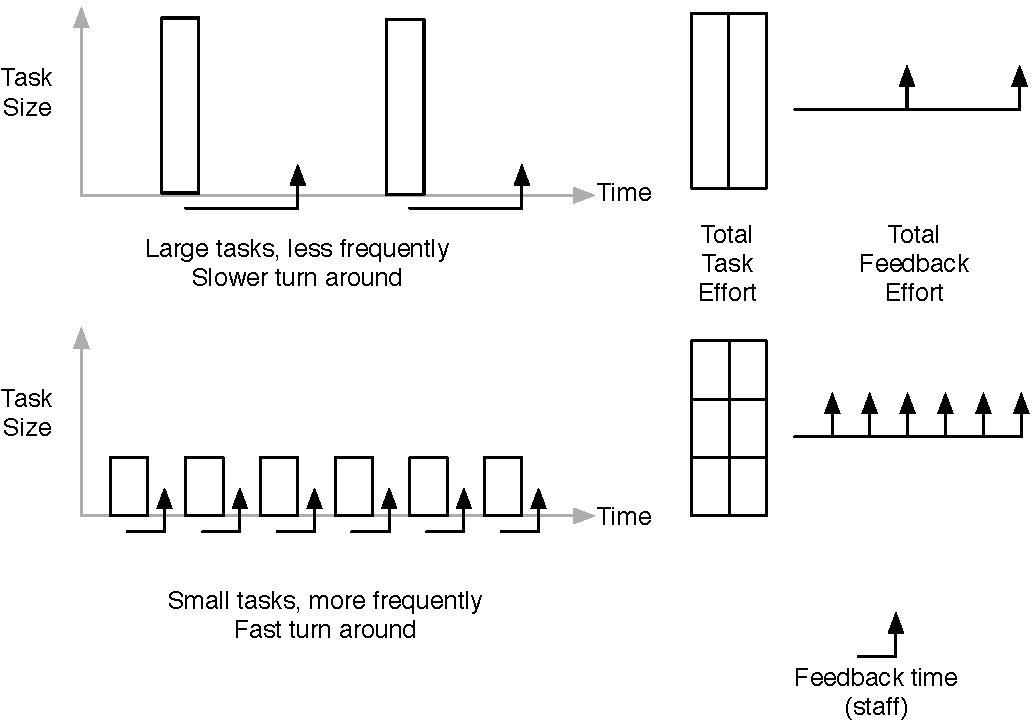
\includegraphics[width=0.8\textwidth]{FormativeFeedback}
	\caption{Illustration of time allocation to assessment tasks, with rectangle areas representing effort expended by staff providing feedback or students preparing submissions.}
	\label{fig:formative_feedback}
\end{figure}

The second issue listed above relates to the assessment of student understanding, in addition to product outcomes. This is particularly relevant to programming units, where it is easy to assess the programs students create rather than attempting to assess their understanding. Assessing product outcomes alone encourages surface approaches to learning, as it is the product and not the understanding that is being assessed. Including some tasks that require students to articulate their understanding provides opportunities for students to engage appropriate cognitive levels, helping them develop the required understanding, while also communicating the importance of this understanding to the students. In this way, these tasks help to encourage students to appropriately engage with learning activities, and to use deep approaches to learning.

The final issue relates to the use of summative assessment, rather than formative feedback, during the teaching period. Including summative assessment in this manner breaks several critical aspects of the approach presented. Assessing the tasks within the teaching period means that an overall assessment of student learning outcomes is no longer possible. This was experienced in one of the early iterations discussed in \cref{cha:evaluation}, with results failing to match outcomes demonstrated in student portfolios.

Using summative assessment during the teaching period also limits the likelihood of students incorporating feedback they receive. Summative assessment is, by its very nature, final, and so students are not encouraged to learn from this assessment. One of the positive aspects of using formative feedback during the delivery of the example units was that understanding became the key focus. Tasks were not complete until students had demonstrated the required understanding. There was no punishment for not having understood an aspect of a topic on the first attempt, freeing teaching staff to provide relevant feedback and guide students toward the required understandings.

While summative assessment during the teaching period works against the overall principles stated in \cref{cha:guiding_principles}, the distinction between formative feedback and summative assessment changes when using summative assessment that aims to provide a qualitative, holistic, assessment of student outcomes. Constructive learning theories require staff to gain an understanding of the likely level of understanding students have developed in order to provide formative feedback. As a result, teaching staff could potentially provide summative assessment of student performances at any stage during the teaching period. In effect, the assessment at the end of the teaching period represents an arbitrary point in time at which this assessment does occur. Ideally, additional flexibility in education could allow this point to be adjusted for individual students further catering for a wide range of capabilities.

Formative feedback with qualitative, holistic, summative assessment of student outcomes is seen as critical to the success of the approach presented in this thesis.

% subsection assessing_learning_outcomes (end)

\subsection{Supporting Principles} % (fold)
\label{sub:supporting_principles}

As shown in \fref{fig:adjusted_how_principles}, principles \ref{itm:focus} to \ref{itm:reflect} can be considered as providing underlying support for the central principles related to the adoption of constructive learning theories, alignment of curriculum, and assessment of learning outcomes. While embracing these principles helps support the central principles, it is possible that alternatives could offer similar outcomes.

\begin{figure}[htbp]
	\centering
	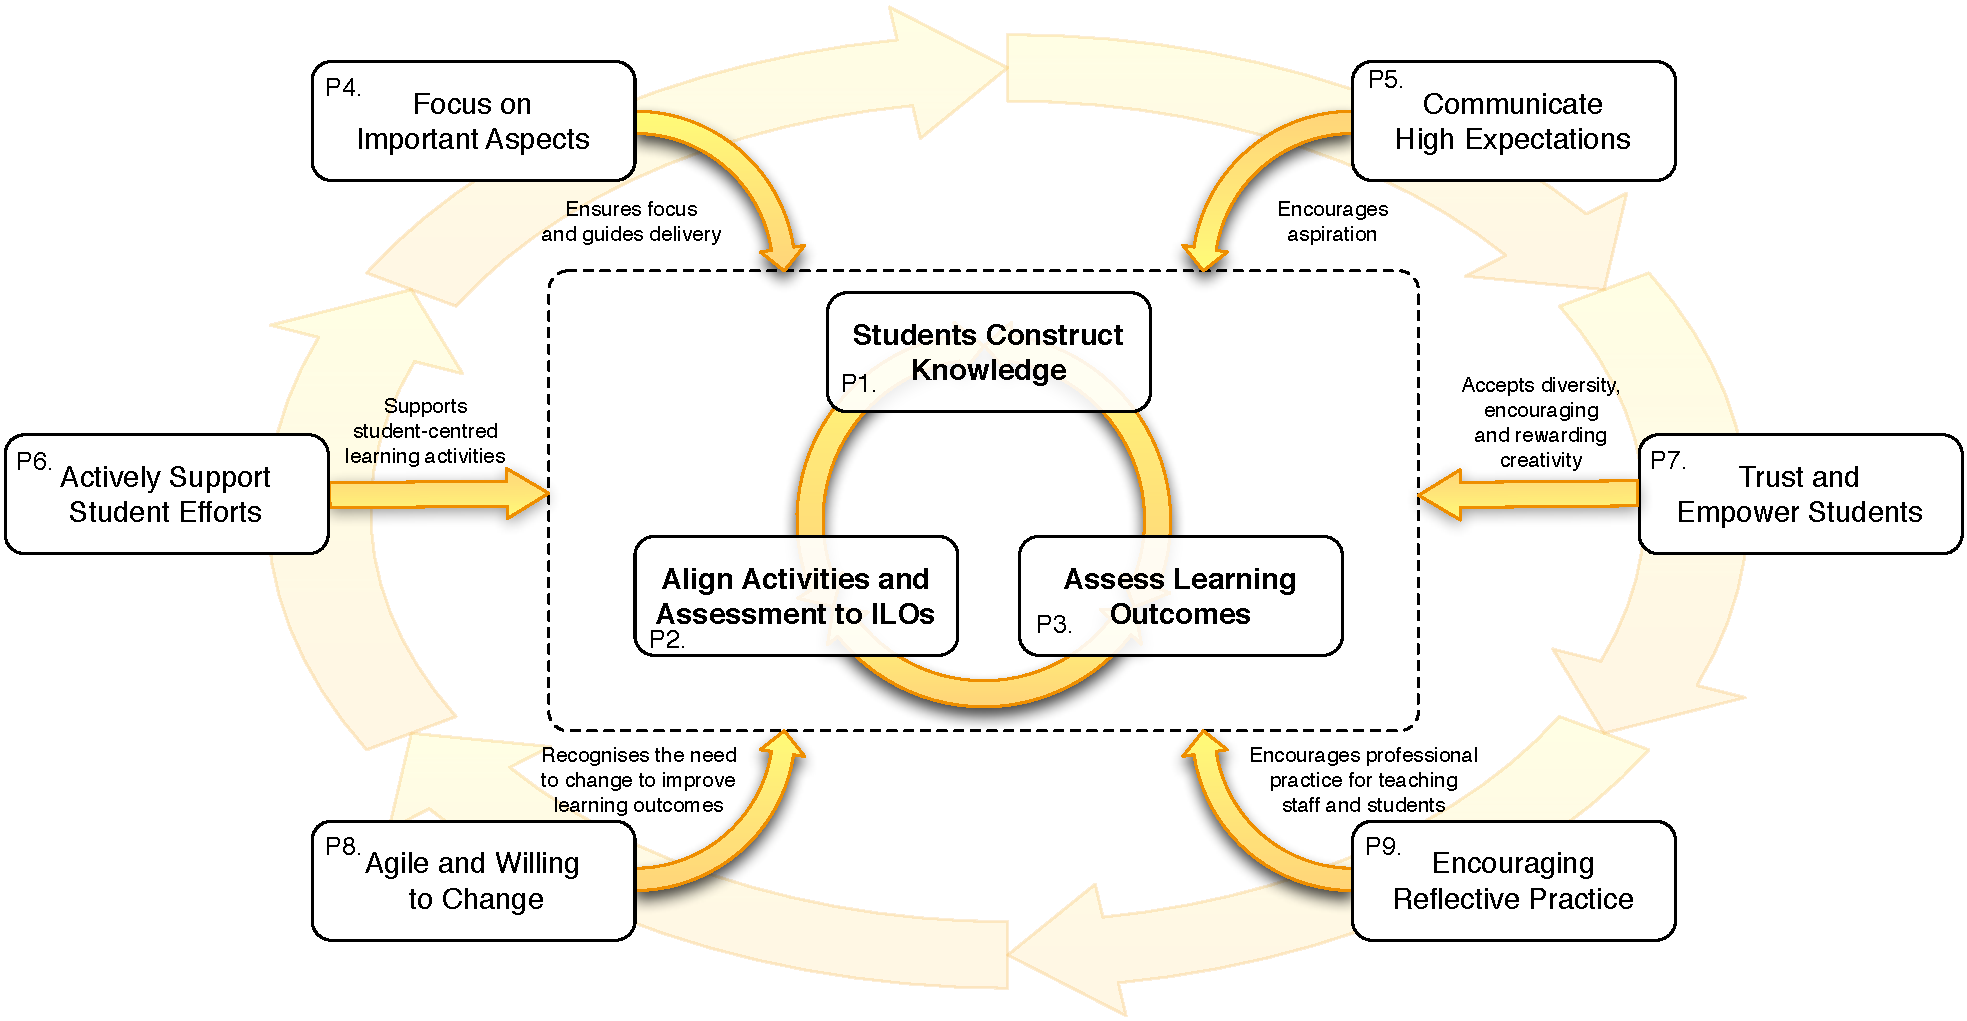
\includegraphics[width=\textwidth]{HowPrinciples}
	\caption{An alternative view of the principles outlined in \cref{cha:guiding_principles}, showing Principles \ref{itm:focus} to \ref{itm:reflect} providing support for the central principles of constructive learning theories, alignment of curriculum, and assessment of learning outcomes.}
	\label{fig:adjusted_how_principles}
\end{figure}

\pref{itm:focus} encourages a focus on communicating only key concepts, and providing students with access to details which they can use as needed. This principle was instrumental in the shift of content from lectures to teaching and learning resources, an approach that also resulted in lighter weight teaching and learning activities that made it easier to make iterative improvements in line with \pref{itm:agile}. If this principle had not been embedded within the example units then the shift away from teacher-focused lectures, to more constructive activities with greater student engagement, would have been more challenging.

\pref{itm:expectations} encourages teaching staff to communicate high expectations to their students, in an effort to promote deep learning. Staff expectations are communicated through the assessment tasks and feedback, with an iterative process, involving frequent formative feedback, being ideally suited for students to respond positively to this encouragement. In the example units, high expectations were communicated throughout the iterative process, with work only being signed off when it was completed to a high standard. The handling of tests in the example units is a particularly relevant case, with students needing to work on improving their answers even when they had successfully completed most of the test questions. Had these high expectations not been communicated students are likely to lower their internal expectations, as was encountered in the first few iterations discussed \cref{cha:evaluation}.

\pref{itm:support} aims to actively support student efforts. When constructive learning theories are adopted, teaching staff can no longer \emph{tell} students what they need to know, instead staff need to \emph{guide} students in their learning. Additional assistance helps students develop their understanding as they attempt to engage with learning activities. With challenging unit content, such as in introductory programming units, this support helps ensure a larger number of students will successfully complete the unit. Where this support is not provided results are likely to suffer, either in terms of overall expectations or number of students successfully completing the unit. 

\pref{itm:theory_y} indicates a need to view students as being genuinely motivated to learn, a Theory-Y view of education. Where this principle is not held, staff are likely to resist the move from summative assessment during the teaching period to formative feedback. Theory-X strategies of coercions and punitive assessment need to be avoided for the benefits of formative feedback to be realised.

\pref{itm:agile} recognises the need to be agile and willing to change. The iterative development of the example units reported in \cref{cha:evaluation} provide a clear demonstration of the value of this principle. In many regards, initial implementations of portfolio assessment were seen as failures, but by embracing change iterative improvements resulted in the positive learning environment experienced in later iterations. Where change is not embraced, situations are not likely to improve on their own. However, once the approach taken does result in good learning outcomes, the need for change reduces.    

Finally, \pref{itm:reflect} encourages the use of reflection by both staff and students. Students are encouraged to reflect on their learning, while staff reflect on student outcome and use this feedback to direct change. Reflection worked hand-in-hand with \pref{itm:agile} in shaping the units outlined in \cref{cha:example_impl}, as reported in \cref{cha:evaluation}. Failing to incorporate this principle would lessen the impact on any change. Similarly, failing to encourage students to reflect on their learning does not take full advantage of the learning environment created.

% \subsection{Embed Reflective Practice} % (fold)
% \label{sub:embed_reflective_practice}

% subsection embed_reflective_practice (end)

% subsection supporting_principles (end)


\subsection{Principles related to ``What'' we teach} % (fold)
\label{sub:principles_related_to_}

In addition to the nine principles related to ``how'' we teach, \cref{cha:guiding_principles} presented three principles on ``what'' we teach. These aimed to work together with the ``how'' principles to create an effective environment for students learning introductory programming concepts. As each of these principles relates specifically to teaching introductory programming, they may not be relevant to teaching other units. This also implies that these principles need not even be addressed by other introductory programming units.

\pref{itm:paradigm} indicates that introductory programming units should aim to communicate a  consistent set of programming concepts centred upon a programming paradigm. In the example units presented in \cref{cha:example_impl}, the procedural paradigm was used in the formation of the introductory programming unit, while object oriented programming principles were focused upon in a second unit. While this selection, and order, of paradigms could be adjusted, it would be hard to imagine an introductory unit that did not centre on an in-depth coverage of a single paradigm.  

Each paradigm centres around a number of programming abstractions, with programs being conceptually constructed through the abstract definition and configuration of these abstractions. \pref{itm:concepts} encourages educators to focus on communicating these conceptual structures, and associated programming concepts. Associated concepts, such as DuBoulay's notional machine \cite{DuBoulay:1986}, then become the focus, rather than the specifics of a programming language's syntax. The realisation of this principle enabled the example units to introduce students to a range of programming languages, helping them better understand the underlying concepts. 

While this concept focus was important for these units, \pref{itm:concepts} is not critical to the the overall approach. Ideally educators should aim to communicate underlying concepts, as these provide students with a broader understanding of programming in general. Where depth in a single language is desired, this could still be achieved with a focus on concepts. So there is little reason not to adopt this principle, though it does require a certain level of expertise from teaching staff, and availability of resources for students to use as they learn the syntax themselves.   

Finally, \pref{itm:authentic} advocates for appropriate use of programming languages. Constructive learning theories indicate that the goal of education is to help students ``think and act'' like experts. This necessitates the \emph{appropriate} use of the tools, and concepts, in teaching and learning activities. By not adhering to this principle, students learn how \emph{not to} do something. This is likely to result in students developing inappropriate understandings of how the relevant tools or concepts should function. These understandings must then be unlearnt before students are able to ``think and act'' as experts. If \pref{itm:concepts} is embraced, then there should be no reason to consider using programming languages in ways other than they were intended.

% subsection principles_related_to_ (end)

\subsection{Applying the Principles for Other Units} % (fold)
\label{sub:applying_the_principles_for_other_units}

\sref{sec:general_applicability_of_constructive_alignment} discussed the general applicability of the approach presented in \cref{cha:approach}, which embodies all of the principles from \cref{cha:guiding_principles}. The general nature of principles 1 to 9 indicate that these can be applied to a range of units. Principles 10 to 12 were formulated to be specific to introductory programming and, as discussed in \sref{sub:principles_related_to_}, would not directly apply to teaching units related to other topics. However, these generalising these three principles provides some insight into how similar principles could be devised for other contexts.

\pref{itm:paradigm} exists due to the goal of introductory programming of enabling students to develop programs. This goal requires that students develop functioning knowledge of associated concepts, and be able to take on the role of a developer. In embodying this role, students must develop a mindset guided by the chosen programming paradigm. Requiring students to change this mindset part way through the teaching period is likely to be highly disruptive to the cognitive structures students have developed. As a result, generalised forms of this principle are only likely to be relevant where a unit aims to develop functioning knowledge in topic area with alternate mindsets. In these cases, the general form of \pref{itm:paradigm} would suggest that, in order to develop depth of understanding, units should focus on introducing students to a single mindset.

The practical nature of software development often means that it is easy to focus on details of syntax, and ignore underlying concepts. In terms of programming, \citet{Winslow:1996} indicated that experts tended to focus on generalised concepts, an observation that is likely to apply in other context as underlying concepts provide experts with the knowledge required to function in a wide variety of circumstances. The generalised aim of \pref{itm:concepts} is, therefore, likely to apply across a range of topic areas as it encourages a focus on these underlying concepts.Similarly, a generalised focus on appropriate use of concepts and tools, as reflected in \pref{itm:authentic}, is also likely to be widely applicable.

% subsection applying_the_principles_for_other_units (end)

% \subsection{Relationships Between Principles} % (fold)
% \label{sub:relationships_between_principles}

% \begin{table}
% 	\begin{tabular}{c|c|c|c|c|c|c|c|c|c|c|c|c}
% 		~ & \Pref{itm:construct} & \Pref{itm:align} & \Pref{itm:formative} & \Pref{itm:focus} & \Pref{itm:expectations} & \Pref{itm:support} & \Pref{itm:theory_y} & \Pref{itm:agile} & \Pref{itm:reflect} & \Pref{itm:paradigm} & \Pref{itm:concepts} & \Pref{itm:authentic} \\
% 		\hline
% 		\Pref{itm:construct}	& & & & & & & & & \\	
% 		\Pref{itm:align}		& & & & & & & & & \\
% 		\Pref{itm:formative}	& & & & & & & & & \\	
% 		\Pref{itm:focus}		& & & & & & & & & \\
% 		\Pref{itm:expectations}	& & & & & & & & & \\	
% 		\Pref{itm:support}		& & & & & & & & & \\
% 		\Pref{itm:theory_y}		& & & & & & & & & \\
% 		\Pref{itm:agile}		& & & & & & & & & \\
% 		\Pref{itm:reflect}		& & & & & & & & & \\
% 		\Pref{itm:paradigm}		& & & & & & & & & \\
% 		\Pref{itm:concepts}		& & & & & & & & & \\
% 		\Pref{itm:authentic}	& & & & & & & & & \\	
% 	\end{tabular}
% \end{table}

% subsection relationships_between_principles (end)


% Basically discuss the impact of removing each of the principles from CH3 individually. Reinforce the notion that they work together. 

\section{Approach in Review} % (fold)
\label{sec:approach_in_review}

\cref{cha:approach} described an approach to delivering constructively aligned introductory programming units that embodied all of the principles from \cref{cha:guiding_principles}. The approach outlined the overall strategy taken, and a number of processes used to create effective learning environments. As discussed in \sref{sec:general_applicability_of_constructive_alignment}, it is believed that this approach can be generalised beyond the context of introductory programming. To illustrate this point, and discuss the critical aspects of this model, this section outlines which aspects of the overall strategy, and which processes, are likely to be needed to recreate an effective learning environment in other contexts.

\subsection{Overall Strategy} % (fold)
\label{sub:overall_strategy}

\sref{sec:overall_strategy} described the overall strategy used to underpin the development and delivery of the unit discussed in \cref{cha:example_impl}. This strategy centred around the use of portfolio assessment as an assessment approach, and a variety of  student-centred delivery approaches to help embed constructive learning theories in unit delivery. This section discusses these decisions, and if and how alternatives could be incorporated.

\subsubsection{Portfolio Assessment} % (fold)
 \label{ssub:portfolio_assessment}

Biggs early work on constructive alignment \cite{Biggs:1996c,Biggs:1999} strongly advocated for the use of portfolio assessment. \citet{Biggs:2007} provides a range of alternative means of implementing constructive alignment under the premise that portfolio assessment is not applicable for large class sizes. However, as shown in \cref{cha:evaluation}, our approach has been able to scale from teaching tens of students in early iteration, to hundreds of students in later iterations through the implementation of the principles described in \cref{cha:guiding_principles}.

Alternative assessment schemes involving the use of summative assessment during the teaching period, and examinations at its end, are not going to be able to reproduce the same ``web of consistency'' as they break several of the core principles outlined in \cref{cha:guiding_principles}. Existing work reporting on applications of constructive alignment are largely representative of this situation, with the large majority still producing students final grade as a combination of arbitrarily weighted assignments and exams. It is, therefore, not surprising that \emph{none} reported having experienced a system with the consistency and alignment as reported by \cite{Biggs:1996c}. 

There are three areas for mismatches between traditional assessment approach using assignments, and the portfolio approach presented in this thesis: frequency of feedback, type of assessment, and contribution to final grade. The approach presented in \cref{cha:approach} advocates the use of frequent feedback, which is formative in nature, and does not directly relate to final graded. With traditional assignments, feedback tends to be in larger blocks, assessment is summative, and some form of weighting needs to be applied to map results to a final grade. Each of these breaks the focus on learning that is achieved using the portfolio approach.

For example, a greater use of formative feedback could be achieved through permitting students to resubmit assignment work after receiving initial results. This is likely to improve unit results, but does not necessarily result in deeper learning. Where assessment remains quantitative, permitting resubmission may inadvertantly encourage shallow learning, as students can adjust assignments to meet marking criteria rather than working toward demonstrating deeper understanding. Similarly, feedback is less relevant if it is not given frequently. Finally, the summative marks from the multiple assignments needs to be combined together, losing the clear link between levels of achievement and final grades that can be achieved through portfolio assessment.

Teaching staff believe that the learning environment experienced as part of this work was only possible due to the shift to portfolio assessment. Portfolio assessment is seen as central to recreating the ``web of consistency'' reported by \citet{Biggs:1996c,Biggs:1999}. 

Consider a unit that assesses students using two essays and a final examination. In order to shift to portfolio assessment, with frequent formative feedback, these assessment tasks could be broken down into a number of smaller tasks, with students receiving feedback at each stage. It is likely that these larger assessment tasks included a number of smaller activities; tasks that staff \emph{assumed} students would perform. Making these the weekly tasks ensures students actually perform the required activities, while also providing artefacts that staff can use to provide students with feedback.

These smaller tasks would form the basis of the Pass and Credit criteria for the unit. To balance workload, the scope or scale of these may need to be adjusted, with the expectation that students would perform the task to a high standard in order to achieve a passing grade. The two essays may become the required artefacts for the Pass and Credit criteria, or could potentially become the Distinction criteria with output from the smaller tasks making up the Pass and Credit grades.

Where an essay was still desired, subtasks could require students to demonstrate understanding of relevant background reading material, to prepare outlines for the final essay, and possibly to perform a peer review of other student work. An example set of subtasks is shown in the following list. 

\begin{enumerate}[noitemsep,nolistsep]
	\item Read background material, and summarise in the form of a blog entry on ``\emph{insert topic}''.
	\item Prepare a draft outline of essay on ``\emph{insert topic}'', which incorporates references from background reading material.
	\item Prepare complete draft version of essay on ``\emph{insert topic}''.
	\item Write a peer review of two other student's work on ``\emph{insert topic}''. 
	\item Submit final version for assessment in portfolio, along with peer reviews and reflections on alterations made.
\end{enumerate}

By completing these tasks, staff would have multiple opportunities to guide student learning, ensuring that the resulting essays are likely to demonstrate students have attained at least the Pass grade standard. 

Frequent student interaction would also help to address potential staff workload issues, as staff aim to provide a small amount of feedback on each of the subtasks. Blog entries could be quickly scanned to see that students had captured critical aspects from each of the reading tasks, outlines could be quickly checked to ensure appropriate structure, while more detailed feedback would need to be provided on completed drafts. Each of these could be marked off in a task tracking system like Doubtfire when they had been completed to a satisfactory standard. Assessing the portfolio would then involved checking that work had been marked off, and considering the changes students had made in response to peer feedback.

Tasks appropriate for Distinction and High Distinction would also need to be considered, and staff and student workloads balanced with the core tasks. Distinction tasks can be devised by teaching staff asking themselves what they \emph{really} want student to be able to do by the end of the unit. In the case of the programming units this resulted in the Distinction criteria requiring students to demonstrate the ability to create a program that demonstrated an appropriate application of the unit concepts. This could involve developing mathematical models for units on mathematics, preparing financial reports in units on accounting, or explaining metabolic processes in units on biochemistry, for example. Assessment criteria can then be defined to require students to perform these tasks in order to achieve Distinction and High Distinction grades.


 % subsubsection portfolio_assessment (end) 

\subsubsection{Delivery Approach} % (fold)
\label{ssub:delivery_approach}

\sref{sec:overall_strategy} also outlined the incorporation of constructive learning theories into the teaching and learning activities using the Beyond Bullet Points approach for lecture presentations, interactive lecture demonstrations, and laboratory sessions with lab, core, and  optional tasks. While each of these was seen as effective in the delivery of the example units, other units are likely to need to use different strategies. 

In deciding upon a delivery strategy, teaching staff would need to consider tasks that are likely to actively involve students in constructing their own knowledge. Where previous activities had relied upon knowledge transmission, such as the standard lecture, these would need to be redesigned with constructivist ideals in mind.

Consider again the hypothetical unit, with the essay assignments and exam now broken down into a number of smaller tasks. The overall strategy for delivering the unit should consider kinds of activities that are likely to be the most effective in ensuring students can achieve the tasks successfully. Using this strategy, the design of the activities themselves need to support students as they complete these tasks, providing them with guidance on associated concepts, tools, techniques, and approaches.

% subsubsection delivery_approach (end)
% subsection overall_strategy (end)

\subsection{Processes within the Model} % (fold)
\label{sub:processes_within_the_model}

After outlining the overall strategy taken in this work, \cref{cha:approach} presented the model of constructive alignment used, and described a number of processed that existed within this model. Given the use of portfolio assessment, a central aspect of the model as outlined in \sref{ssub:portfolio_assessment}, these processes are likely to be appropriate for the delivery of a number of portfolio based units. For teaching staff, the model presented the following processes:

\begin{enumerate}[noitemsep,nolistsep]
	\item Define Intended Learning Outcomes
	\item Construct Assessment Criteria
	\item Develop Teaching and Learning Activities and Resources
	\item Deliver Unit
	\item Provide Feedback and Guidance
	\item Assess Student Portfolios
\end{enumerate}

Each of these processes is going to be essential in delivering any unit using constructive alignment and portfolio assessment. Intended learning outcomes need to be stated using active verbs, which can be drawn from the SOLO Taxonomy. These outcomes then become the central focus for unit, with students aiming to demonstrate they have achieved these outcomes in their portfolios. Assessment criteria need to define performance objectives for each grade outcome, and indicate the kinds of evidence students need to submit. Teaching and learning activities and resources need to be develop, or existing activities and resources used. Delivery of the unit will need to incorporate frequent formative feedback to ensure that students work is likely to meet intended learning outcomes, and student portfolios need to be assessed in order to determine final student grades. 

With the hypothetical unit all of these processes would be relevant. Intended learning outcomes and assessment criteria would need to be defined, or re-examined, using the guidelines from \sref{sub:defining_intended_learning_outcomes} and \sref{sub:constructing_assessment_criteria}. Teaching and learning activities would be designed with the aim of best helping students to achieve the intended learning outcomes, as planned by staff with the core tasks in the assessment work. Iterative delivery would permit students to receive feedback on their progress, while also providing staff with a clear picture of student progress and potential areas of misunderstandings. Finally, student work can be captured in their portfolios and assessed against the criteria set out at the start of the unit.

% Where differences can occur, is in details of how these processes are performed.

% \cref{cha:approach} described a number of guidelines for defining intended learning outcomes for a programming unit. The relevance of each of these is discussed in the following list. 
% \begin{itemize}[noitemsep,nolistsep]
% 	\item \loref{lo-solo} recommended the use of the SOLO taxonomy as a reference point for selecting appropriate verbs, and this is likely to also be relevant for other units. 
% 	\item \loref{lo-know-prog} indicated that the outcomes should include both conceptual knowledge, and programming competencies. For other units, a similar mix of objectives requiring declarative and functioning knowledge is likely to be applicable.
% 	\item \loref{lo-simple-terms} suggested that intended learning outcomes should be expressed using simple terms, a suggestion that should apply to any units looking to use this approach.
% 	\item \loref{lo-minimal} advised the use of a small number of intended learning outcomes, incorporating prior research and experiences reported from Iteration 1 in \cref{cha:evaluation}.
% 	\item \loref{lo-general} and \loref{lo-flex} indicated that intended learning outcomes should be general and flexible enough to allow students to have some creativity in how they address the outcomes.
% \end{itemize}


% subsection processes_within_the_model (end)





% What from the Approach can change?
% - Portfolio Assessment?
% - Delivery Approach?
% - Guidelines? (CH4)


% section approach_in_review (end)

% Could you do it differently?

% No frequent formative feedback = heavy workload to assess portfolios (a little each week, or lots at the end) little each week as added benefits of improved learning, lots at the end ???

% section approach_and_principles_in_review (end)

% \section{Risk Assessment of Approach} % (fold)
% \label{sec:risk_assessment_of_approach}



% \subsection{Surface Learning and Plagiarism} % (fold)
% \label{sub:surface_learning_and_plagiarism}

% Risks:
% \begin{itemize}[noitemsep,nolistsep]
% 	\item Plagiarism of core tasks.
% 	\item Details are missed by rapidly assessing portfolios.
% \end{itemize}

% % subsection surface_learning_and_plagiarism (end)

% \subsection{Staff and Student Workloads} % (fold)
% \label{sub:staff_and_student_workloads}

% % subsection staff_and_student_workloads (end)

% % section risk_assessment_of_approach (end)



% 4: Risk Assessment of Approach

% How does the approach address risks related to "Surface Learning and Plagiarism" (subsection 1) and "Staff and Student Workloads" (subsection 2).



% section reflection_on_findings_and_experience (end)

\section{Challenges for Wider Adoption} % (fold)
\label{sec:challenges_for_wider_adoption}

\subsection{Adopting Constructive Learning Theories} %It is easier to be a ``Sage on the stage'' than a ``Guide by the side''} % (fold)
\label{sub:adopting_constructive_learning_theories}

Constructivist learning theories are central to the principles and approach outlined in this thesis. This requires that educators adopt key aspects of constructivism as their theory-in-use, not just their espoused theory \cite{Argyris:1976}. A shift from a primarily objectivist view of education, to one centred on constructive learning theories requires a significant conceptual change, and is likely to be one of the large challenges to the wider adoption of this approach.  

Objectivist views provide educators with a number of convenient truths. Knowledge transfer is conceptually simple: get a number of people in a room and tell them what they need to know. Guiding students in the construction of their own knowledge seems like a much greater challenge. Accepting the students central role in constructing their own knowledge, means rethinking old strategies, and looking for new ways to engage students with the material. 

Constructivist learning theories require a move from teacher-centred to student-centred learning environments, which in turn requires educator to release some control of the learning environment. With teacher-centred activities, such as lectures, teaching staff have complete control of the content, pace, and method of delivery. With traditional lectures there is the possibility for well scripted lectures to be delivered by teaching staff who are not experts in the area. As more student-centred activities are adopted there is a need to incorporate greater input from students, enabling them to shape the environment to their needs. This requires teaching staff who are able to dynamically adjust delivery, ensuring the direction and focus of class activities are likely to result in productive learning for as many students as possible. Teaching staff need to be experts of the subject matter, as well as likely student misconceptions and strategies to address those misconceptions.

% subsection adopting_constructive_learning_theories (end)

\subsection{Releasing Control of Assessment} % (fold)
\label{sub:releasing_control_of_assessment}

Another significant challenge is the required release of control over the assessment process, with the loss of ``marks'' as a means to motivate students. As noted in \cref{cha:evaluation} (Iteration 2) one of the great challenges in implementing this Theory-Y based approach had been the anxiety of teaching staff over this perceived loss of control. Common, Theory-X based, wisdom indicates that students only work on items allocated marks. If you want students to \emph{do} some task, then that task must be allocated marks. With this view, marks are the ``carrot and stick'' for educators wanting to motivate students. Abolishing the practice of allocating summative marks during the teaching period abandons this common wisdom, and requires a Theory-Y based perspective of student motivation.

As with the shift to constructive learning theories, abandoning marks is a large challenge. The structured literature review in \cref{cha:background} indicated that most reported applications of constructive alignment had adopted constructive learning theories for teaching and learning activities, but that assignments and exams remained the dominant assessment strategy. Moving away from the common wisdom in this regards appears to be a larger challenge than accepting constructive learning theories.

Part of this challenge is addressing educators prior experiences, a result of the self-fulfilling nature of the Theory-X focus on marks. Students want to achieve a good result from the unit, and unit grades provide an externally visible measure of this performance. Marks are awarded for successfully completing tasks, and these marks directly relate to the grade students will achieve. Consider the case where laboratory tasks are unmarked, and assignments marked. In this situation students are encouraged by the marks to focus on the assignment work, despite the valuable learning that may have taken place if they did other tasks. Any staff member using combinations of marked and unmarked work will have experienced this focus, leading to the common wisdom that students only focus on tasks that have marks associated with them.

% subsection releasing_control_of_assessment (end)

\subsection{Holistic Assessment over Piece-by-Piece Assessment} % (fold)
\label{sub:holistic_assessment_over_piece_by_piece_assessment}

The approach to portfolio assessment described in \cref{cha:approach} also aims to holistically evaluate student learning outcomes, the core of \pref{itm:formative}. This goes against the common education practice of allocating percentages to each artefact a student submits, and determining their final result from a combination of these weighted tasks. With the approach presented in this thesis, it is the intended learning outcomes together with the assessment criteria that determine final grades, not the artefacts themselves. Using the portfolio assessment scheme outlined in this thesis requires a change in thinking about how students are assessed overall.

Consider the portfolio assessment of the Research Project unit. This unit required students to undertake a research project, and to submit a portfolio that consisted of a research proposal and plan, research report, artefacts associated with an oral presentation, a learning summary report, and other artefacts relevant to the student's project. Given this list of required components, traditional approaches would seek to allocate percentages to each of these components. In contrast, applying the guidelines from \cref{cha:approach} requires the definition of standards of achievement for the different grade outcomes, with the artefacts acting as the student's evidence of their ability to meet the intended learning outcomes.

While this may be understood by the academics involved in the teaching of the unit, this distinction also needs to be communicated to administrators and other academic staff who oversee unit accreditation. Units delivered using the approach recommended in this thesis are likely to stand out as being ``different'', with a greater chance of encountering resistance despite good pedagogical foundations. Overcoming these obstacles is likely to require some levels of support at a larger institutional level. 

% subsection holistic_assessment_over_piece_by_piece_assessment (end)

\subsection{Perceived Workload Issues} % (fold)
\label{sub:perceived_workload_issues}

Frequent formative feedback and portfolio assessment have the appearance of requiring significant extra work for staff, and students, making it easy to dismiss as impractical. Teaching staff do need to be given sufficient time to engage with students, but as outlined in \sref{sub:assessing_learning_outcomes} this need not result in significant extra effort. Time taken to \emph{mark} assignments now goes into providing formative feedback, and time allocated to \emph{mark} exams goes to \emph{grading} portfolios. Efficiencies can the gained through reflective practice, with each iteration aiming to improve staff, and student, productivity by ensuring teaching and learning activities meet student needs.

% subsection perceived_workload_issues (end)

\clearpage
\subsection{Availability of Experienced Teaching Staff} % (fold)
\label{sub:availability_of_teaching_staff}

Units are typically taught by a team of teaching staff, including lecturers and tutors for example. When the approach is first implemented at a given institute, there is not likely to be any teaching staff who have experience with this approach. This adds additional overhead for the first few iterations, as staff and students learn about the new teaching and learning environment.

% subsection availability_of_teaching_staff (end)



\subsection{Combined Issues} % (fold)
\label{sub:combined_issues}

Constructive alignment with portfolio assessment, as outlined in this thesis, helps create a productive student-centred teaching and learning environment, but\ldots it is easy to find a reason \emph{not} to implement this approach. Change is hard, and the approach presented in \cref{cha:approach} requires teaching staff adopt key constructive learning theories, a Theory-Y perspective of student motivation, and abandon the common use of marked assignments for holistic assessment of a body of work against set criteria. Then, once an individual academic has made this transition there are potential institutional barriers that need to be overcome to allow the approach to be implemented. 

\tref{tbl:common_reasons} indicates the common reasons given for not being able to consider using an approach similar to the one presented in this thesis. Most of the reasons given are not valid, and those that are reflect a disconnect with current research into effective educational practice. Change is difficult, but there is no good reason not to consider implementing the approach presented in this thesis to a range of technical and non-technical units.

\begin{table}[p]
	\centering	
	\caption{Common reasons for rejecting the approach, their validity and relevance. }
	\label{tbl:common_reasons}
	\begin{tabular}{p{5.5cm}|c|p{6cm}}
		\textbf{Reason for Rejecting} & \textbf{Valid} & \textbf{Relevance} \\
		\hline
		\emph{I can't run interactive lectures} 	& Yes   & Constructivist learning theories are not likely to be easy to apply. \\
		\emph{Will not scale} 						& No    & It will scale, if care is taken. \\
		\emph{Student won't work without marks} 	& No    & Experience shows otherwise, real learning requires it. \\
		\emph{Need good tutors} 					& Yes   & When are good tutors not required? \\
		\emph{Need new material} 					& Maybe & Material does need to align to intended learning outcomes. \\
		\emph{Need weighted tasks} 					& No    & Portfolios enable holistic criterion referenced assessment. \\
		\emph{Need norm-referenced assessment} 		& No    & Best practice indicates otherwise. \\
		\emph{No detailed marking scheme} 			& No    & Do need detailed assessment criteria. \\
		\emph{It's subjective} 						& No    & Criteria must be objectively specified and applied. \\
		\emph{Only people with prior experience can get high marks} & No & Students with a range of backgrounds have been able to achieve Distinction and High Distinction results. \\
		\emph{Requires too much of students} 		& No    & This requires only that students demonstrate they have achieved the stated unit learning outcomes. \\
		\emph{Requires too much of staff}			& No 	& If quality education is the goal, then staff need to be allocated sufficient time to provide student feedback. \\
		\emph{Requires students to write}  			& Yes   & Student need to be able to communicate their understandings. \\
		\emph{Too different / hard} 				& Yes / No & It is different, but once understood and in place it is easier.\\
	\end{tabular}
\end{table}

Once the approach is implemented it is also important to realise that any change of this nature is likely to require a number of iterations before the true benefits are realised. In many cases it is expected that the first iterations are likely to encounter unexpected difficulties, as was the case with the implementation of this approach in Iterations 1 and 2 as discussed in \cref{cha:evaluation}. Once the approach is undertaken, it will require a degree of persistence to see the implementation through to productive outcomes. 

Given these tight constraints, it will be challenging to promote this approach for wider adoption. However, as parts of the approach, such as the use of constructive learning theories in delivering teaching and learning activities, slowly gain in popularity, the chance of others adopting this approach improves.

% subsection combined_issues (end)

% section challenges_for_wider_adoption (end)



% 6: Overall Outcomes

\section{Overall Outcomes} % (fold)
\label{sec:overall_outcomes}

Teaching staff currently delivering the portfolio assessed units, as outlined in \cref{cha:example_impl}, aim to continue using this approach. The approach is credited with enabling the positive, student-centred, supportive teaching and learning environment, which improves with each iteration. In this environment any student who makes a genuine attempt at learning the associated concepts is likely to succeed. Having a clearly set goal, as stated by the intended learning outcomes and assessment criteria, in the unit outline means that staff and student are working \emph{together} to help students achieve the best results possible.

Removing marks clearly communicates the importance of \emph{understanding} the associated concepts (\Pref{itm:formative}) with each student receiving individual feedback on things they need to concentrate on. Frequent formative feedback help point students in the right direction, with their tasks being signed off once they have demonstrated the associated understanding. Working though these activities helps develop student understanding (\Pref{itm:construct}) of related concepts (\Pref{itm:align}) and builds their confidence, helping them believe in their own potential and encouraging them to aim high (\Pref{itm:expectations}).

Interactive teaching and learning activities create a feeling of mutual respect between students and staff (\Pref{itm:construct}, \Pref{itm:align}, and \Pref{itm:theory_y}). Students inputs and questions actively shape the learning environment, with opportunities to explore their questions and to address their misconceptions. Classroom sessions are an opportunity to explore ideas, and for students to develop a better understanding of the important aspects and focus for each weeks work (\Pref{itm:focus}). Teaching staff provide support (\Pref{itm:support}) and guidance, helping students construct their knowledge (\Pref{itm:construct}), rather than being a source of knowledge that needs to be transferred to the students. Creating a environment which values both teacher staff and students. 

The flexibility of the portfolio assessment empowers students to take responsibility for their own learning (\Pref{itm:theory_y}), encouraging and rewarding students for focusing on developing their understanding of the unit's concepts (\Pref{itm:construct} and \Pref{itm:align}). The grades students achieve are based upon their effort and capability, not on how well their study aligned with the questions staff selected for an exam. Student can explore a wide range of aspects related to the unit, engage their creativity and imagination, and be rewarded for this. 

Embracing Theory-Y based assessment practices that encourage appropriate behaviour, rather than punish inappropriate behaviour, ensures a positive and collaborative learning environment (\Pref{itm:theory_y}). The use of constructive alignment with portfolio assessment in the example units discussed in \cref{cha:example_impl} yielded all of the positive experiences reported by \citet{Markwell:2004}, with students becoming more active in the learning environment as delivery improved with each iteration.

Open assessment of learning outcomes also removes the hidden ceiling imposed by traditional assignments and exams, enabling the environment to support a much wider range of capabilities. While students who struggle to understand the material can aim to achieve at least the passing criteria, those who have developed the required understanding can go beyond these tasks and demonstrate their own individual learning achievements. The environment pushes everyone, from the struggling students to the high achieving students, asking them all to learn as much as they can and to demonstrate this understanding at the end of the unit. 

Tasks that push the high achieving students do not discourage struggling students, as these are not required to pass. In fact, the open nature of these tasks means those who are undertaking them encourage others to strive to achieve the required understanding to achieve these results themselves. Seeing others work on projects they are really interested in, and seeing them succeed is a powerful motivating factor, and once a struggling student constructs a more viable model of the units concepts, they too can start to engage with these more challenging tasks. In this way the system ensures that all students are encouraged to learn and strive to achieve excellence (\Pref{itm:expectations}) throughout the teaching period.   

Reflective practice, with a focus on important aspects and a willingness to change, helps ensure that each delivery of a unit improves upon the last (\Pref{itm:focus}, \Pref{itm:agile}, and \Pref{itm:reflect}). Focusing on teaching and learning activities, and what they ask the students to do, provides a means of guiding students through tasks likely to assist them in the construction of their own knowledge (\Pref{itm:construct} and \Pref{itm:focus}). Maintaining this focus throughout the design, development, and delivery of the unit gives students the best opportunity to develop the required understandings (\Pref{itm:construct} and \Pref{itm:align}).

When teaching introductory programming, the procedural and object oriented paradigms (\Pref{itm:paradigm}) provide central themes around which to base the unit. Each paradigm offering its own concepts and principles around which the unit's tasks can centre (\Pref{itm:concepts}). Helping students develop appropriate skills with associated languages (\Pref{itm:authentic}).

All of the hard work from students and staff in a given teaching period then culminates in the portfolio assessment. Students work, which has been developed under the guidance of staff, is collected together in each student's portfolio, and presented for assessment. Student's pride in their achievement is palpable, with the portfolio representing a physical embodiment of many hours of hard work.

Portfolio assessment is also one of the highlights for teaching staff. While Pass and Credit portfolios demonstrate suitable knowledge in the subject matter, the Distinction and High Distinction portfolios are always full of astounding work. Students take the freedom given to them and run with it, achieving things that could not have been expected of them. Interviewing these students is always a pleasure, and an opportunity for teaching staff to engage with the most gifted and hard working students.

The main challenge with teaching introductory programming using this approach, has been to motivate students who do not feel they should be learning to program. These students actively work against learning the material, with some desperately wanting to retain shallow approaches to learning that do not succeed with this approach. For these students, the challenge is not in teaching the material but in helping motivate them to genuinely attempt the tasks. The work of \citet{Guzdial:2005} provides some indication of strategies that may succeed with these students, though in this case it is engineering students who do not see the relevance of programming to their career outcomes. 

Overall, teaching environments created using the approach presented in this thesis are focused on students developing their understanding. Summative assessment is reduced in favour of formative feedback, and closed punitive assessment strategies are replaced with open encouraging strategies that aim to help students achieve their best possible result. This does require support from teaching staff, but that is rewarded by the quality of the work students are able to achieve. 

% section overall_outcomes (end)

\section{Future Work} % (fold)
\label{sec:future_work}

This thesis represents a start, rather than end, of a range of research opportunities. Having developed the principles and approach across a number of iterations, there is now opportunities to further investigate portfolios collected, and to examine ongoing changes in the activities used and their impact on student results.

Work to date have collected hundreds of student portfolios, each of which captures an individuals learning outcomes from their engagement with the teaching and learning environment. While some analysis has been performed on these portfolios there are many other opportunities that can now be exploited. Student reflections, their programs, reports, custom projects, and research reports all provide different opportunities to explore aspects of the teaching and learning environment from student perspectives.

While student portfolios have demonstrated their ability to create programs, it would be very interesting to repeat an experiment similar to that conducted by \citet{McCracken:2001}. The mathematical nature of the exercises should be changed to better reflect the more general nature of the programming units, but otherwise it would be interesting to evaluate students ability to implement a set specification. Where students were unable to get the program working, it would be interesting to extend the experiment to determine the likely cause of the problem, and the extent of help needed for the student to succeed in implementing the program. This would help improve understanding of the limitation of students at the end of their first year of programming, and likely assistance they will need in implementing programs on their own. 

Longitudinal studies could examine how students from early portfolio units progress through later units. Does this experience help them succeed at other programming units? Do students feel they learnt more general skills they could apply to a wider range of units, or was the learning entirely focused on programming knowledge? How do portfolio assessed units relate to other units, from the students perspective? What differences can they identify? Would students like to see more portfolio units? Interviewing students at the end of their degree programme could provide a deeper understanding of what is working, and what can be improved with the proposed approach.

In the broader context, future work is needed to trial the approach in other contexts, and other educational institutes. It would be interesting to see how well the approach can be adapted to non-technical units, where there may be additional challenges in identifying how frequent formative feedback can be achieved. Where the principles from \cref{cha:guiding_principles} can be adopted, it is believed that similar positive learning outcomes will be achieved.

While \sref{sec:challenges_for_wider_adoption} outlined some of the challenges believed to faced this wider adoption, a more systematic analysis of peoples responses to the approach would also be enlightening. The approach is believed to be genuinely better than alternatives, but discussions with others have been met with general resistance. Better understanding people's doubts about the approach could help adapt strategies to more effectively encourage people to consider its use.

Once wider adoption has been achieve, it would be interesting to compare learning outcomes from units using constructive alignment with portfolio assessment, from those using more traditional forms of assessment. By examining a range of units, in different contexts, it should be possible to gain some comparative statistics to support the qualitative findings from this work.

% section future_work (end)

\section{Discussion Summary} % (fold)
\label{sec:disc_summary}

This chapter provided a discussion of the approach presented in this thesis, and its underlying principles. The general applicability of the approach was discussed, indicating that it should be able to apply beyond the context of introductory programming to a wider range of educational contexts. The importance of each of the principles was outlined, along with a discussion of the likely impact of ignoring each principle on the resulting teaching and learning environment, indicating that key aspects from the principles are required for benefits to be realised. Similarly, the critical importance of the portfolio assessment and constructive learning theories in guiding the delivery approach were also discussed.

Challenges facing wider adoption are numerous, as the delivery and assessment approach differ from education norms. Where these challenges can be overcome, an effective teaching and learning environment can be achieved, one that encourages and rewards students for focusing on developing deep understanding. In this environment, students engage their imagination and creativity in meeting the unit's intended learning outcomes, while staff focus on providing student with guidance and feedback. The results, better learning opportunities for students that push them no matter what their level of understanding.

% section discussion_summary (end)


% Is it all worth it?
% What changes have been observed?

% - Supportive environment focused on learning
% - Students are empowered to engage their creativity and imagination
% - Widening of perspective - support students in a wider range of activities
% - Supporting a wider range of capabilities
% -- No upper bound on what can be learnt (and given credit for)
% -- While still catering for 
% - Encourages interaction between staff and students -- interviews give you access to the best students (and gets them talking to us)

% 7: Other Points of Interest


% 8: Future Work



% \section{Other Points of Discussion} % (fold)
% \label{sec:other_points_of_discussion}



% % Some smaller points of discussion:
% % - Use of Pascal to remove focus from syntax (support existing work)
% % - Objects First / Objects Later and the Paradigm Shift
% % - Failing Students and Student Motivation (link to Guzdial work on non-majors)


% % - Success of Resources -- short/specific had longer life, separation of resources useful
% Short/specific podcasts had a longer life

% Concept podcasts were not as successful... more resources?

% Separation of activities and resources? - successfull


% % section other_points_of_discussion (end)


% \subsection{Related work on general education principles} % (fold)
% \label{ssub:related_work_on_education_principles}

% %
% % JG - I am not sure about this section in terms of fit & content...
% %
% % Maybe could incorporate in the principles sections???
% %
% %


% In discussing how to improve undergraduate education, \citet{Chickering:1987} listed seven principles for good practice in undergraduate education. These are practices that:
% \begin{enumerate}[noitemsep,nolistsep]
% 	\item Encourages contact between students and faculty.
% 	\item Develops reciprocity and cooperation among students
% 	\item Encourages active learning
% 	\item Gives prompt feedback
% 	\item Emphasizes time on task
% 	\item Communicates high expectations
% 	\item Respects diverse talents and ways of learning
% \end{enumerate}

% The following list states how each of the principles from \citet{Chickering:1987} are integrated with the principles underlying this work. 
% \begin{itemize}[noitemsep,nolistsep]
% 	\item The strong emphasis on frequent formative feedback should be used to help encourage contact between students and faculty. (\Pref{itm:formative}, \Pref{itm:support})
% 	\item This same formative process should also be harnessed to encourage sharing and cooperation amongst students. (\Pref{itm:formative},\Pref{itm:support},\Pref{itm:theory_y})
% 	\item The central nature of the students in constructing their knowledge necessitates an approach that encourages active learning. (\Pref{itm:construct},\Pref{itm:theory_y})
% 	\item The formative feedback process needs to ensure that work is returned promptly to students, ensuring they receive the feedback while it is still relevant. (\Pref{itm:formative})
% 	\item Communicating high expectations is included directly in our principles. (\Pref{itm:expectations})
% 	\item Assessment and teaching and learning activities need to be flexible, enabling different styles of learning and to engage with students diverse talents. (\Pref{itm:support})
% \end{itemize}





% \section{Future Work} % (fold)
% \label{sec:future_work}

% Structured Literature review - interesting to note referencing in the field

% Formally evaluate the time taken

% Compare the reliability of assessment

% \citet{Guzdial:2005} non-majors


% section future_work (end)

% chapter discussion (end)